\chapter{System analysis in the Z domain}
	Until now to describe a \textbf{discrete-time time-invariant linear system} (using techniques in the time domain) two dual alternatives were presented:
	\begin{itemize}
		\item using the \de{impulse response} $h(n)$ of the system in order to determine the output as the convolution with such sequence with the input, so $y(n) =  x(n) * h(n)$;
		\item using the \de{linear} and \de{constant difference equation} \textbf{LCDE} obtained by the discretization of the differential operator that allows to sequentially/numerically generate a sequence that can be solved for the new output $y(n)$ depending on the previous inputs/outputs:
		\begin{equation}
			\sum_{k=0}^N a_k\, y(n-k) = \sum_{k=0}^M b_k\, x(n-k)
		\end{equation}
	\end{itemize}

	This dual formulations was presented in the example of section \ref{sec:ex:lowpass} where the passive low-pass filter was characterized by both the impulse response
	\[ h(n) = ba^n u(n) \hspace{2cm} \textrm{with } a = \frac{1}{1 + \frac{T_s}{RC}}\quad b = 1-a \]
	as well as finite difference
	\[ y(n) = a\, y(n-1) + b\, x(n) \]
	
	As we can see discrete-time LTI systems can be univocally described by this different (but still equally characterizing of the problem) methods; in particular it will be shown that performing an analysis of the system in the Z domain this two representation will be somehow \textit{merged}.
	
\section{Z transform}
	The \de{Z transform} can be regarded as the Laplace transform for discrete-time functions $x(n)$ that are described in the domain of the \textbf{complex variable} $z\in \mathds C$; the definition of the transform is
	\begin{equation}
		X(z) = \Z{x(n)} := \infsum n x(n) z^{-n} \quad \in \mathds C
	\end{equation}
	We define also the \de{region of convergence} $ROC$ as the subset of the complex plane $\mathds C$ on which the Z transform of the function $x(n)$ converges to a finite value.
	
	\paragraph{Transform of the exponential sequence} Given the exponential sequence defined by the function $x(n) = a^n$ it's easy to observe that
	\begin{align*}
		\textrm{if } a > 1 \qquad &\Rightarrow \quad \sum_{n=0}^\infty a^n = \infty  \\
		\textrm{if } 0 < a < 1 \qquad &\Rightarrow \quad \sum_{n=-\infty}^0 a^n = \infty
	\end{align*}
	and so the Z transform will always diverges, determining an empty set for the region of convergence.
	
	Considering instead a \textbf{causal exponential sequence} $x(n) = a^n u(n)$, the application of the Z transform will result in the expression
	\begin{equation} \label{eq:z:causaleexponential}
	\begin{aligned}
		X(z) & = \infsum n a^nu(n) z^{-n} = \sum_{n=0}^\infty a^n z^{-n} = \sum_{n=0}^{\infty} \left( \frac a z\right)^n  \\
		& = \frac{1}{1-az^{-1}}
	\end{aligned}
	\end{equation}
	In this case the transform has been obtained only for the values of $a$ that allows to have a convergent series that in this case requires of having $\left|\frac az\right| < 1$; for this reason the region of convergence of the causal exponential sequence is
	\begin{equation}
		ROC = \big\{ z \in \mathds C \textrm{ such that } |z| > |a| \big\}
	\end{equation}
	From a geometrical point of view, the region of convergence is determined by all the points in the $z$ plane that are lying outside the circle of radius $a$.
	
	Considering now the \textbf{anti-causal} exponential sequence $x(n) = -a^n u(-n-1)$ it can be proven that it's Z transform is still the one described by equation \ref{eq:z:causaleexponential} with with the complementary region of convergence:
	\begin{equation}
		X(z) = \frac{1}{1-az^{-1}} \hspace{2cm} \textrm{with } ROC = \big\{ z \in \mathds C \textrm{ such that } |z| < |a| \big\}
	\end{equation}

	\paragraph{Relation with the DTFT} Considering the definition of the \dtft (described by equation \ref{eq:four:dtft}, page \pageref{eq:four:dtft}) it's possible to observe a similarity with the Z transform; in particular the DTFT is the evaluation of the Z transform around the unit circle, in fact
	\begin{equation}
		X\big(e^{j\omega}\big) = X(z) \Big|_{z=e^{j\omega}}
	\end{equation}
	
	This concept is similar to the relation between the \ctft and the Laplace transform where the first is the evaluation of the second along the imaginary axis:
	\[ X(\Omega) = X(s) \Big|_{s=j\Omega} \]
	
	\paragraph{Inversion} To invert the Z transform and retrieve a discrete-time sequence we can use the definition
	\begin{equation}
		x(n) = \mathcal Z^1\left\{ X(z) \right\} := \frac{1}{2\pi j} \oint_\Gamma X(z) z^n\, dz
	\end{equation}
	where $\Gamma$ is any closed loop in the region of convergence routed in anti-clockwise direction.
	
	\subsection{Properties}
		\paragraph{Linearity} Similarly to the Laplace and Fourier, also the Z transform is a linear operator and in particular we have that
		\begin{equation}
			\Z{a\, x(n) + b\, y(n) } = a \Z{x(n)} + b \Z{y(n)} \qquad \forall a,b\in \mathds R
		\end{equation}
		and the region of convergence of the so computed transform is the intersection of the region of convergence of the initial sequences:
		\[ ROC_{x+y} = ROC_x \cap ROC_y \]
		
		\paragraph{Time shifting and time reversal} The time shifting property allows to compute the Z transform of a signal $x(n)$ shifted in time by $n_0$ samples knowing it's initial transform $X(z)$ using the formula
		\begin{equation}
			x(n-n_0) \quad \mapsto \quad z^{-n_0} X(z)
		\end{equation}
		For this reason a block containing a term $z^{-d}$ for diagram representation of system relates to a delay of the output of $d$ samples.  The time reversal property instead states
		\begin{equation}
			x(-n) \quad \mapsto \quad X(z^{-1})
		\end{equation}
		
		\paragraph{Multiplication by an exponential} For every coefficient $\alpha \in \mathds R$ we have that
		\begin{equation}
			\alpha^nx(n) \quad \mapsto \quad X\left( \frac z \alpha \right)
		\end{equation}
		
		\paragraph{Convolution} For the Z transform also the convolution theorem still holds stating that
		\begin{equation}
			y(n) = x(n) * h(n) \quad \mapsto \quad Y(z) = X(z)H(z)
		\end{equation}
	
\section{Transfer function}
	As was presented at the start of this chapter, the dual representation of discrete-time time-invariant linear system can be merged in the Z domain considering the following relations:
	\begin{equation}
		Y(z) = X(z)H(z) \hspace{1.5cm} \leftrightarrow \hspace{1.5cm} \sum_{k=0}^N a_k z^{-k} Y(z) = \sum_{k=0}^M b_k z^{-k} X(z)
	\end{equation}
	This two representation can collapse in the same definition of the \de{transfer function} $H(z)$ of the system that can be regarded as a \textbf{rational polynomial} in the variable $z^{-1}$:
	\begin{equation}
		H(z) = \frac{Y(z)}{X(z)} = \frac{\sum_{k=0}^M b_k z^{-k}}{\sum_{k=0}^N a_k z^{-k}}
	\end{equation}
	
	If the transfer function $H(z)$ is real evaluated, then it means that all the coefficients $a_i,b_i$ are also real evaluated; the numerator presents $M$ roots called \textbf{zeros} while the denominator has $N$ roots called \textbf{poles}. We can observe that if the transfer function diverges, this is due to a pole with a value of 0 (the division by 0 in fact diverges).
	
	\paragraph{Zero poles transfer function} Considering a transfer function with $N=0$ poles, the impulse response of the system is finite with a length of $M$ samples, in fact by computing the inverse Z transform we can see that
	\begin{equation} \label{eq:z:zeropoles}
		H(z) = \frac{\sum_{k=0}^M b_k z^{-k}}{a_0} = \sum_{k=0}^M \frac{b_k}{a_0} z^{-k} \hspace{1.2cm} \xrightarrow{\mathcal Z^{-1}} \hspace{1.22cm} h(n) = \sum_{k=0}^M b_k\, \delta(n-k)
	\end{equation}
	
	\paragraph{Zero \textit{zeros} transfer function} Considering the other case of a transfer function $M=0$ zeros that can so be written in the form
	\begin{equation}
		H(z) = \frac{b_0}{\sum_{k=0}^N a_k z^{-k}} = \sum_{k=0}^N \frac{b_0}{a_k} z^k 
	\end{equation}
	Such kind of transfer function is typical of infinite impulse response systems.
	
	\subsection{Partial fraction decomposition}
		The fact that the transfer functions are rational polynomial in the variable $z^{-1}$ it means that, depending on the number of zeros/poles, such expression can be split into rational polynomial of lower degree:
		\begin{equation} \label{eq:z:pfd}
			 H(z) = \frac{N(z)}{D(z)} = Q(z) + \frac{R(z)}{D(z)}
		\end{equation}
		In particular the so computed quotient $Q(z)$ present a $M-N$ polynomial degree; in particular, depending on the number of poles/zeros we can classify transfer function discrete-time LTI systems as
		\begin{itemize}
			\item if $M=N$, then $H(z)$ is a \textit{proper} transfer function;
			\item if $M<N$, then $H(z)$ is a \textit{strictly proper} transfer function;
			\item if $M>N$, then $H(z)$ is a \textit{improper} transfer function;
		\end{itemize}
		Only for improper transfer functions the partial function decomposition determine the polynomial quotient $Q(z)$ (of equation \ref{eq:z:pfd}) that's so associated to a finite impulse response (such polynomial in fact can be regarded as a unique transfer function with zero poles as in equation \ref{eq:z:zeropoles}). In general for all cases, the rational polynomial $R(z)/D(z)$ presents $N_p$ number of distinct poles having each multiplicity $m_i$ each that can be rewritten as the sum of \textit{simpler} transfer functions having a single pole each. With this idea equation \ref{eq:z:pfd} can be rewritten using the process of the the so called \de{partial fraction decomposition} in the form
		\begin{equation} \label{eq:z:pfdextended}
			H(z) = \sum_{r=0}^{M-N} B_r z^{-r} + \sum_{i=1}^{N_p} \sum_{k=1}^{m_i} \frac{A_{ik}}{\big(1-p_i z^{-1}\big)^k}
		\end{equation}
		where $p_i$ is the $i$-th pole of the denominator $D(z)$. The collection of the terms $A_{ik}\in \mathds C$ determine the \textbf{residues} of the transfer function; in the case of a transfer function with no multiple poles (so $m_i=1 \forall i$) the terms associated to the residual are all causal exponential sequences and the inversion of equation \ref{eq:z:pfdextended} determines the following impulse response:
		\begin{equation}
			h(n) = \sum_{r=0}^{M-N} B_r \, \delta(n-r) + \sum_{i=0}^N A_i p_i^n u(n)
		\end{equation}
		In this case necessary and sufficient condition for the \textbf{stability} of the causal discrete-time LTI system is that all the poles $p_i$ of the transfer functions have to lie inside the unit circle in the complex domain of the variable $z$.
	
	\subsection{Inverse system}
		
		\begin{figure}[bht]
			\centering 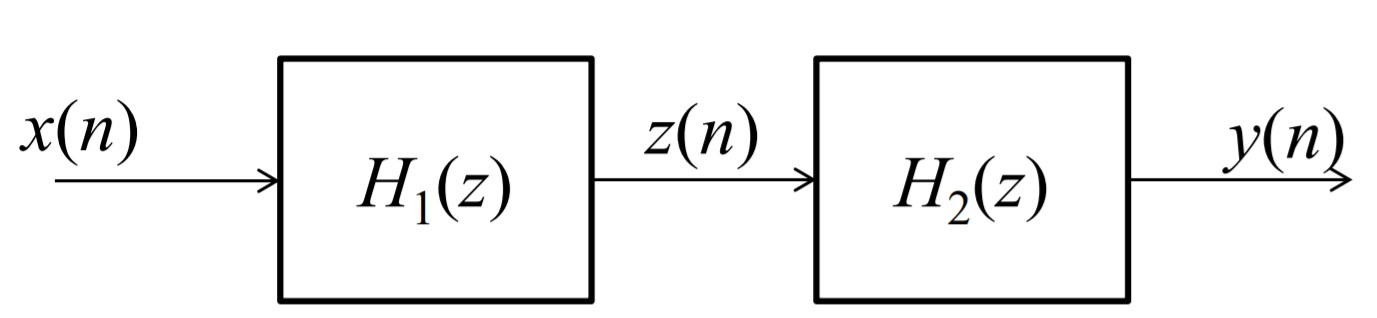
\includegraphics[width=8cm]{doublesystem}
			\caption{cascade of two systems with transfer function $H_1$ and $H_2$, input $x$, intermediate and final output respectively $z,y$.} \label{fig:z:cascade}
		\end{figure}
	
		Considering the case of a cascade of two system as shown in figure \ref{fig:z:cascade}, the output $y(n)$ of the system can be computed as
		\[ y(n) = z(n)*H_2(z) = x(n)*H_1(z) * H_2(z) \hspace{1cm} \xrightarrow{\mathcal Z} \hspace{1cm} Y(z) = X(z)H_1(z)H_2(z) \]
		From this preamble we define transfer function $H_2(z)$ as the \de{inverse} of $H_1(z)$ if and only if 
		\begin{equation}
			H_1(z)H_2(z) = 1 \qquad \Leftrightarrow \qquad H_2(z) = \frac{1}{H_1(z)}
		\end{equation}
		
		Using the stability criterion previously stated, the second system in order to be stable must have poles (namely the zeros of $H_1(z)$) that are lying within the unit circle.\\
		From this a causal and stable LTI system has an inverse that's also causal and stable if and only if all poles and zeros lie inside the unit circle and such system are called \textbf{\textit{minimum phase systems}}.
		
\section{Implementation of LTI systems: signal flow graphs}
	Considering a discrete-time causal LTI system, the numerical processing complexity heavily depends on the algorithmic implementation chosen; assuming to compute the output as the convolution of the impulse response
	\[  y(n) = \sum_{k=0}^\infty h(k) x(n-k)  \]
	then the number of multiplication and addition required linearly increases with the length of the input sequence $x(n)$ and so it's usually not a feasible solution.
	
	Considering instead to use \textbf{finite difference equations} that allows to compute the output in the form
	\begin{equation}
		y(n) = \sum_{k=0}^M \frac{b_k}{a_0} x(n-k) - \sum_{k=1}^N \frac{a_k}{a_0} y(n-k)
	\end{equation}
	the computation requires $M+N$ additions/multiplication for each computed sample (independently from the length of the input sequence $x(n)$); this is usually the preferred way to solve discrete-time systems. The last way to numerically implement such type of systems is by using the transfer function:
	\[ Y(z) = H(z)X(z) \]
	This operation is generally not profitable because it requires the computation of the Z transform ant it's successive inversion.
	
	\subsection*{Block diagrams and signal flow graphs}
		To graphically represent LTI system two equivalent methods can be used: \de{block diagrams} where \textit{blocks} (performing generic operation) are connected by arrows while the other method uses \de{signal flow graph} by having nodes adding weighted edges (the contains in themselves the multiplication); comparison between this two dual representation is shown in figure \ref{fig:z:dualrepresentationgraph}.
	
		\begin{figure}[bht]
			\centering 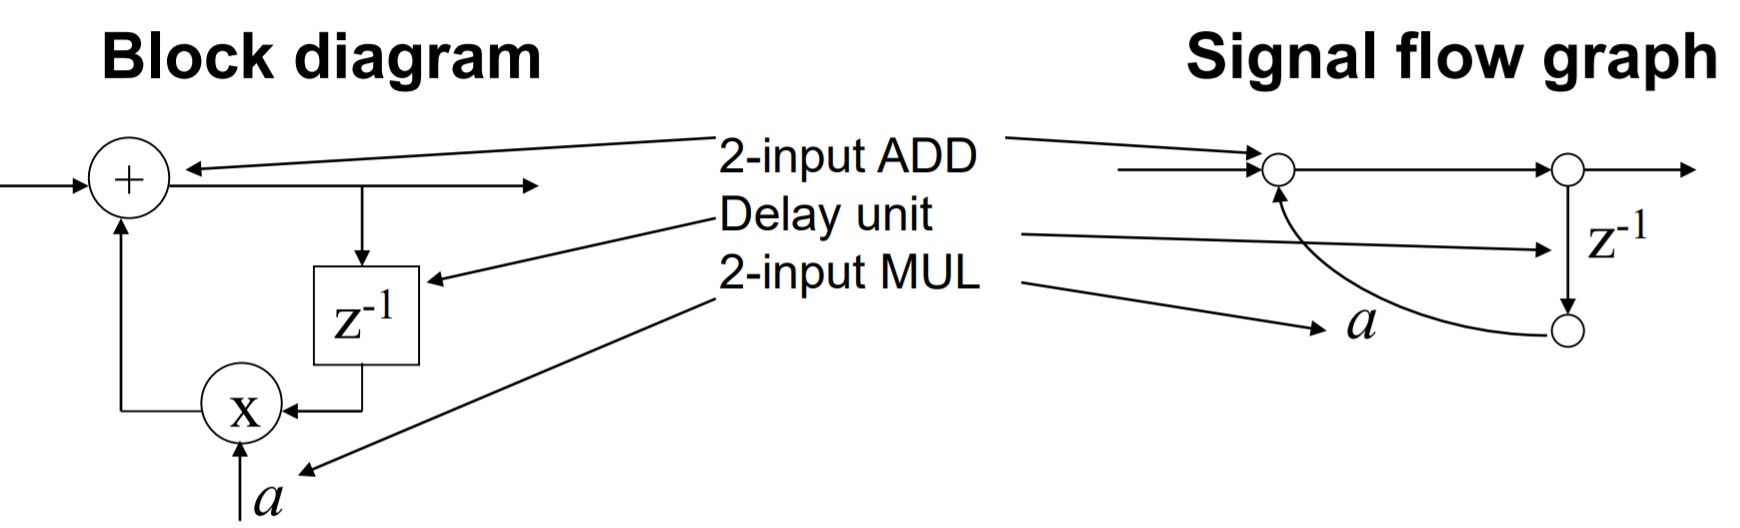
\includegraphics[width=10cm]{graphs}
			\caption{block diagram vs signal flow graph representation and correlation between the various operations performed.} \label{fig:z:dualrepresentationgraph}
		\end{figure}
	
		Such kind of description is useful in digital signal processing because it allows a \textit{good} design and modelling of the system itself before the proper hardware/software implementation. Any discrete-time transfer function can be represented as a flow graph (and using transposition property even more forms can be formulated).
		
		\paragraph{Computable graph} A signal flow graph is referred as \de{computable} if and only if it's possible to compute all the variables of the graph according to a specified order starting from given initial conditions.
		
		Considering as example the graph shown in figure \ref{fig:z:computablegraph} it's possible to define the values of all the edges considering the signals
		\begin{align*}
			w(n) & = x(n) + a \, u(n) \\ z(n) & = w(n) \\ u(n) & = z(n-1) 
		\end{align*}
		hence the output is
		\[y(n) = z(n) = x(n) + a \,y(n-1)\]		
		\begin{SCfigure}[2][bht]
			\centering 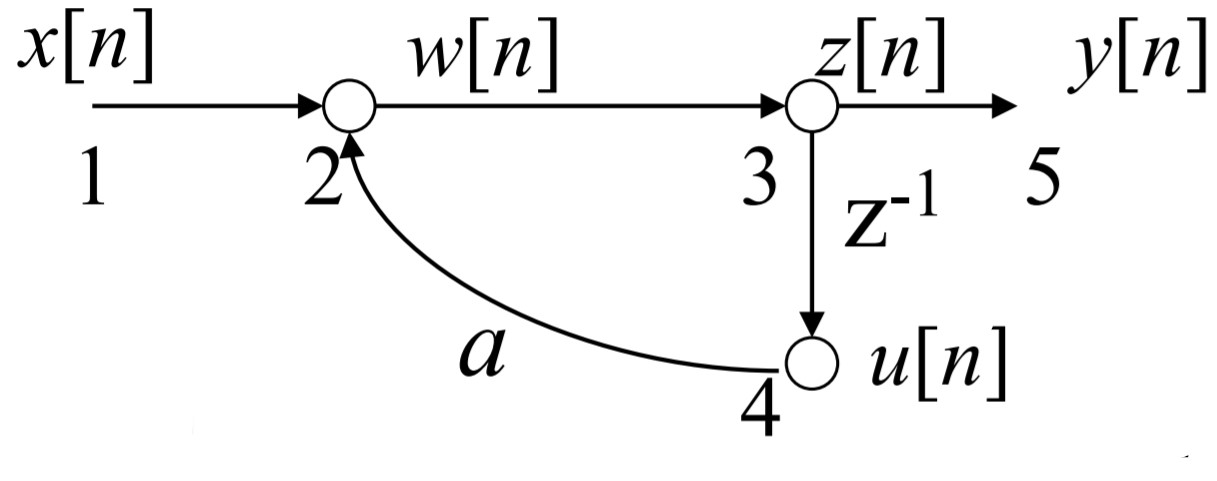
\includegraphics[width=4.5cm]{computegraph}
			\caption{example of computable flow graph.} \label{fig:z:computablegraph}
		\end{SCfigure}
		
		Considering instead the graph in figure \ref{fig:z:noncomputable}, the same analysis gives the signals
		\begin{align*}
			w(n) & = x(n) + a\,z(n) \\ z(n) & = w(n) \\ y(n) & = z(n)
		\end{align*}
		In this case it's impossible to decide whether to compute before the second node (determining $w(n)$) of the third ($z(n)$).	
		\begin{SCfigure}[2][bht]
			\centering 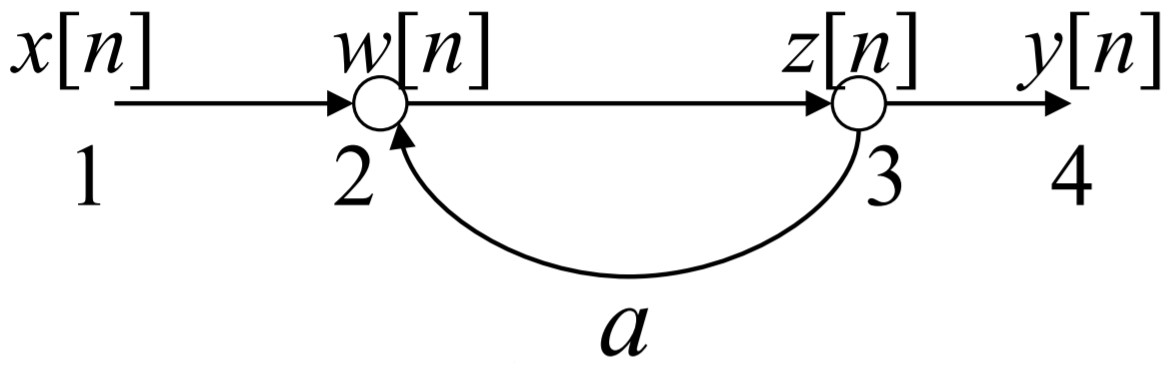
\includegraphics[width=4.5cm]{noncomputable}
			\caption{example of non-computable flow graph.} \label{fig:z:noncomputable}
		\end{SCfigure}
		
		As general \textbf{property} a signal flow graph is computable if and only if each loop in the graph contains at least one delay element.		
		
	\subsection{Direct form I and II}
		As was previously shown, discrete-time LTI systems can be described both in the discrete-time domain using the form
		\[ y(n) = \sum_{k=0}^M b_k x(n-k) - \sum_{k=1}^N a_k y(n-k) \]
		or the dual in the frequency domain
		\[ Y(z) = \dfrac{\sum_{k=0}^{M}b_k z^{-k}}{ 1+ \sum_{k=1}^{N}a_k z^{-k}} X(z) = H_{num}(z) X(z) H_{den}(z) \]
		
		Considering the transfer function $H(z) = H_{num}(z)/H_{den}(z)$ characterized by the polynomial in $z^{-1}$ for the numerator and denominator allows to write the \de{direct form I} of the associated flow graph by \textit{drawing} the \textit{ladders} as shown in figure \ref{fig:z:direct1}. Such implementation requires
		\[ M+N+1 \text{ multiplications} \qquad M+N \text{ additions} \qquad M+N\text{ delays} \]
		
		\begin{SCfigure}[2][bht]
			\centering 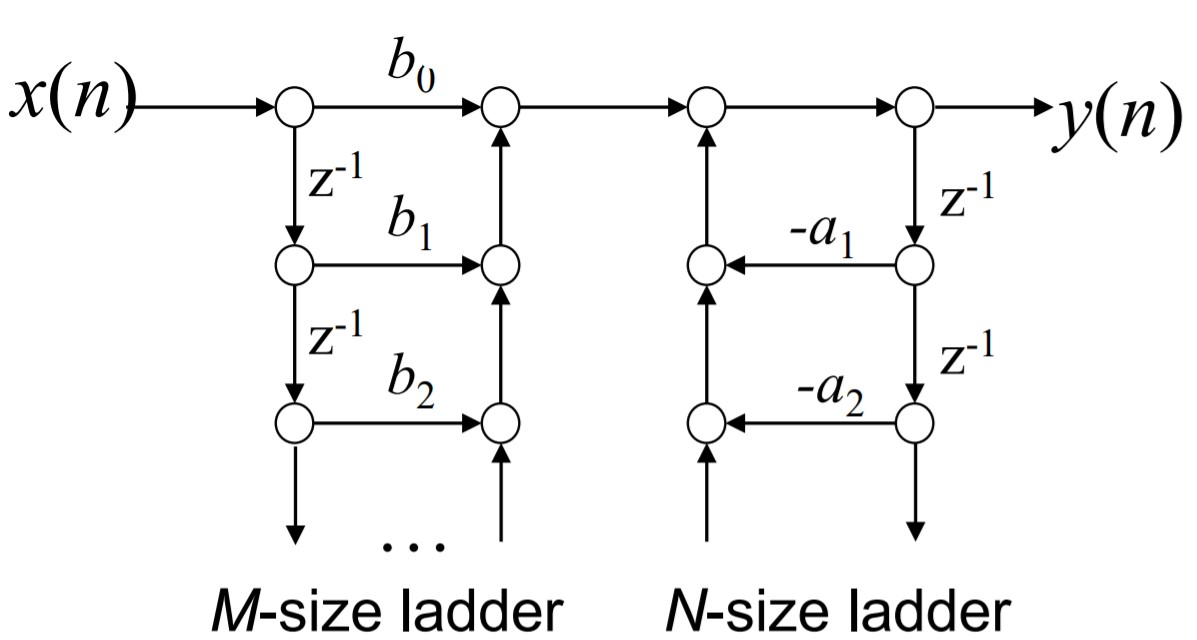
\includegraphics[width=6cm]{direct-form-1}
			\caption{first direct form flow graph representation for discrete-time systems.} \label{fig:z:direct1}
		\end{SCfigure}
	
		To reduce the computational costs of the graph computation we can consider the commutative property of the multiplication, considering so the output as $Y(z) = H_{den}(z) H_{num}(z)X(z)$; this means \textit{swapping} the ladders of the numerator/denominator of the first direct form determining so the \de{direct form II} (or \textbf{canonical}) flow graph representation. As shown in figure \ref{fig:z:direct2}, this \textit{re-arrangement} allows to reduce the delay computations reducing the numerical calculations to
		\[ M+N+1 \text{ multiplications} \qquad M+N \text{ additions} \qquad \max\{ M,N \}\text{ delays} \]
		
		\begin{SCfigure}[2][bht]
			\centering 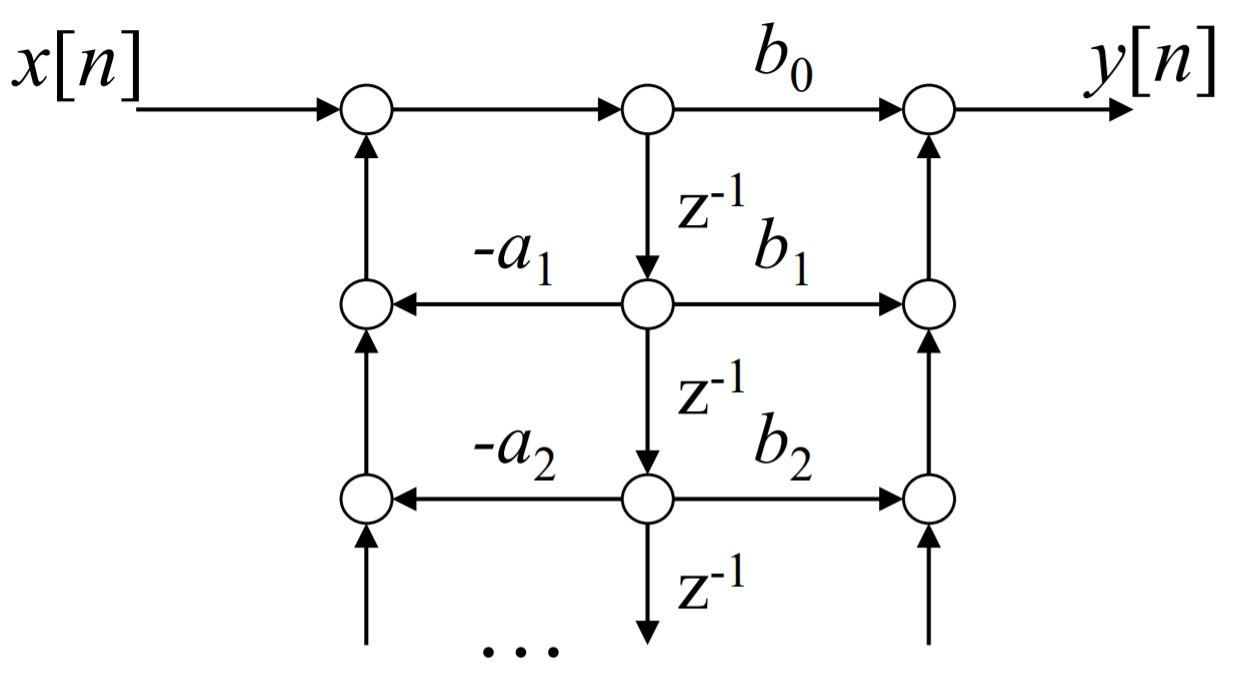
\includegraphics[width=6cm]{direct-form-2}
			\caption{second direct form flow graph representation for discrete-time systems.} \label{fig:z:direct2}
		\end{SCfigure}
		
	\subsection{Transposed form II}
		Transposing the canonical flow graph we obtain the \de{transposed form II} one as shown in figure \ref{fig:z:transposed2}; this implementation still relies on
		\[ M+N+1 \text{ multiplications} \qquad M+N \text{ additions} \qquad \max\{ M,N \}\text{ delays} \]
		but also is naturally \textit{pipelined-oriented}, meaning that is more suitable for hardware (but also software) implementation because long data-paths are broken by registers into shorter data paths.
		
		\begin{SCfigure}[2][bht]
			\centering 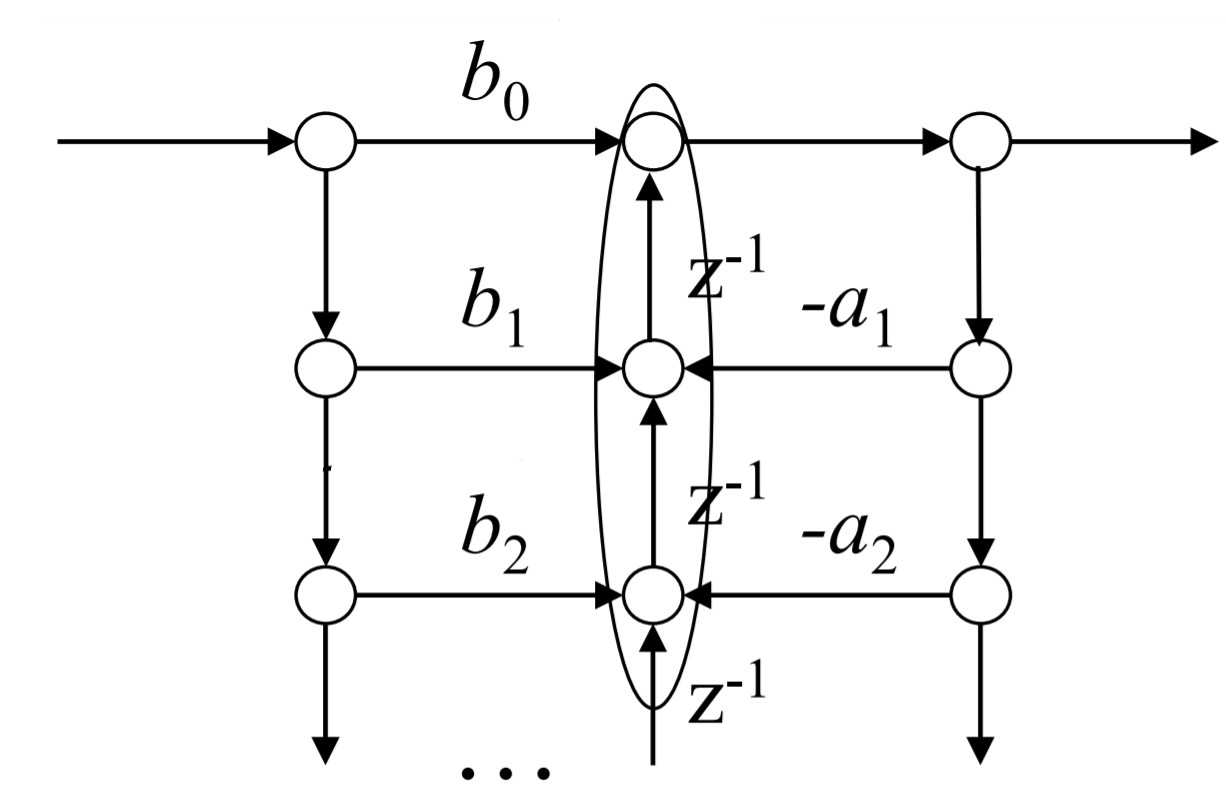
\includegraphics[width=6cm]{transposed-form-2}
			\caption{flow graph of transposed form II obtained as transosition of the canonical graph (figure \ref{fig:z:direct2}).} \label{fig:z:transposed2}
		\end{SCfigure}
		
		
		
		
		
		
		
		
		
		
		
		
		
		
		
		
		
		
		
		
		
		
		
		
		
		